\documentclass[journal,twoside]{IEEEtran}
\usepackage{amsmath,amssymb,amsfonts}
\usepackage{graphicx}
\usepackage{booktabs}
\usepackage{multirow}
\usepackage{xcolor}
\usepackage{cite}
\usepackage[hidelinks]{hyperref}

\newcommand{\ppo}{\textsc{PPO}}
\newcommand{\trpo}{\textsc{TRPO}}
\newcommand{\grpo}{\textsc{GRPO-C}}
\newcommand{\dapo}{\textsc{DAPO-C}}
\newcommand{\eg}{e.g.,\ }
\newcommand{\ie}{i.e.,\ }

\begin{document}

\title{From Trust Regions to Group Baselines: A Unified Empirical Study of
Proximal Policy Optimization Families for Robot Control}

\author{Aitachi%
\thanks{Manuscript generated with the Reinforcement-Learning-Policy open
suite: https://github.com/aitachi/Reinforcement-Learning-Policy. Code,
environments, reward paradigms and raw run logs accompany this paper.}}

\maketitle

\begin{abstract}
Proximal Policy Optimization (\ppo{}) and its relatives dominate practical
robot learning, while Group Relative Policy Optimization (GRPO) and its
successors, developed for large language model (LLM) post-training, replace
the learned critic with an episode-outcome group baseline. These two lines
evolved in disjoint communities with different conventions, and their
relative behaviour on robot control tasks---where samples are expensive and
rewards are engineered---is rarely measured under a controlled protocol. We
present a unified empirical study of twelve algorithms spanning the
trust-region family (\trpo{}, \ppo{}-Clip, adaptive-KL \ppo{}, rollback
variants \ppo{}-RB and TR-\ppo{}-RB, early-stopped ESPO, phasic PPG, and A2C),
the group-relative family (\grpo{}, \dapo{}), and the off-policy anchors
SAC and TD3, on three self-contained vectorized robot tasks of medium difficulty:
2D obstacle-avoidance navigation, planar monopod locomotion with
series-elastic knee dynamics, and 3-link reach--grasp--lift manipulation.
All methods share collection budgets, network sizes, optimizers and
evaluation protocols; each runs under four reward paradigms (sparse, dense,
potential-based, curriculum). Across 189 runs we report final performance,
sample efficiency, seed-level stability, wall-clock cost and
parameter-sensitivity diagnostics. Trust-region safeguards (adaptive KL,
early stopping, trust-region rollback) decide reliability on
contact-rich locomotion, holding seed spread within $\pm$0.12 where plain
clipping scatters to $\pm$0.26; the maximum-entropy off-policy anchor SAC
dominates both smooth navigation (0.83 success) and locomotion
(0.90$\pm$0.001, also the sample-efficiency leader) at 5--8$\times$ the
wall-clock cost, while deterministic TD3 is unreliable across seeds
(0.43$\pm$0.20 on navigation, 0.00 on grasping); and
group-relative methods transfer poorly: with episode-outcome baselines
they reach only 0.32--0.38 success on navigation and near-zero on
locomotion and manipulation under dense rewards, because outcome-level
credit cannot guide multi-stage physical control. Algorithm rankings are
reward-paradigm-dependent---potential-based shaping rescues sparse-reward
training on navigation and grasping yet collapses on locomotion---so
algorithm and reward must be chosen jointly. We release the suite, all
runs and per-term reward audits as an open benchmark connecting LLM
post-training methods back to robot control.
\end{abstract}

\begin{IEEEkeywords}
reinforcement learning, policy optimization, PPO, TRPO, GRPO, DAPO,
robot control, reward design
\end{IEEEkeywords}

\section{Introduction}
Policy gradient methods are the de-facto workhorse of robot learning:
trust-region methods~\cite{schulman2015trpo} established monotonic
improvement guarantees, \ppo{}~\cite{schulman2017ppo} traded those
guarantees for clipped first-order simplicity, and a long line of
variants---rollback clipping~\cite{yuan2020rollback}, early
stopping~\cite{li2023espo}, phasic updates~\cite{cobbe2021ppg}---tuned the
bias/variance of the surrogate objective. Implementation
choices matter as much as the objective~\cite{engstrom2020implementation}.

Independently, the LLM post-training community converged on group-relative
methods: GRPO~\cite{shao2024grpo} removes the critic by baselining a
response against a group of responses sampled from the same prompt, and
DAPO~\cite{yu2025dapo} stabilizes training with clip-higher, dynamic
sampling and outcome filtering. These tricks target LLM-specific
pathologies (low-probability exploration tokens, zero-variance groups,
truncation-polluted outcomes), and it is an open question how they transfer
when the ``token sequence'' is a continuous robot trajectory and the
``outcome reward'' is a physical success event.

This paper measures exactly that transfer under a controlled protocol
(\S\ref{sec:protocol}). We ask three questions:

\begin{enumerate}
\item \textbf{Q1.} Within the trust-region family, which update rule
(clipped, KL-penalized, rollback, trust-region rollback, early-stopped,
phasic) offers the best performance--stability--cost trade-off on robot
control?
\item \textbf{Q2.} Do group-relative methods trained on episode outcomes
remain competitive when the outcome is physical success, and which DAPO
tricks contribute?
\item \textbf{Q3.} How do algorithm ranking and reward paradigm interact:
does the best algorithm depend on the reward signal's density?
\end{enumerate}

Our contributions: (i) a unified implementation of twelve algorithms under
identical budgets and a signal--reward decoupled environment layer; (ii)
three new vectorized robot tasks (obstacle navigation, series-elastic
hopper, kinematic grasp-lift) with four swappable reward paradigms each;
(iii) 189 controlled runs with multi-seed learning curves, stability and
cost metrics; (iv) concrete guidance and an open benchmark.

\section{Related Work}
\subsection{Trust-region and proximal methods}
\trpo{}~\cite{schulman2015trpo} constrains the KL divergence between
consecutive policies and solves a natural-gradient step via conjugate
gradients. \ppo{}~\cite{schulman2017ppo} replaces the constraint with a
clipped probability-ratio surrogate; its adaptive-KL variant tunes a
penalty coefficient online. GAE~\cite{schulman2016gae} controls the
bias/variance of advantage estimation. \ppo{}-RB~\cite{yuan2020rollback}
observes that the flat clipped plateau zeroes gradients for
out-of-band ratios and replaces it with a linear rollback slope;
a trust-region variant triggers the rollback by a per-state KL threshold.
ESPO~\cite{li2023espo} stops inner epochs early when the average
probability-ratio deviation exceeds a threshold, recovering the spirit of
the trust region without a hard clip. PPG~\cite{cobbe2021ppg} separates
policy and value optimization into phases so the shared trunk can absorb
value information without policy interference, anchored by a KL clone term.
Implementation details---value clipping, orthogonal initialization,
learning-rate separation---carry measurable
effects~\cite{engstrom2020implementation,huang2022closer}.

\subsection{Group-relative methods from LLM post-training}
GRPO~\cite{shao2024grpo} (DeepSeekMath) bases each response against its
group and adds a reference-policy KL term; Dr.\,GRPO~\cite{liu2025drgrpo}
removes length and std normalization biases. DAPO~\cite{yu2025dapo}
contributes clip-higher (asymmetric epsilon widening exploration),
dynamic sampling (resampling zero-variance groups), token-level loss and
overlong filtering. GSPO~\cite{qiu2025gspo} replaces sequence-level KL.
These mechanisms assume discrete token actions and verifiable outcome
rewards; adapting them to continuous control requires re-deriving the
grouping (initial states), the clip granularity (timesteps) and the
truncation filter (timeouts), which we make explicit in \S\ref{sec:methods}.

\subsection{Benchmarks and empirical studies}
Atari/MuJoCo studies established protocol design
practices~\cite{henderson2018deep,machado2018revisit}; recent
large-scale replays quantify implementation
sensitivity~\cite{engstrom2020implementation,huang2022closer}. For LLM RL,
open verdicts on GRPO-style training exist~\cite{yu2025dapo,liu2025drgrpo},
but no controlled comparison bridges the two communities on robot tasks;
this work fills that gap.

\section{Preliminaries and a Unified View}
\label{sec:methods}
\subsection{On-policy policy gradients with GAE}
Let $\pi_\theta$ be a tanh-squashed diagonal Gaussian policy
$u\!\sim\!\mathcal{N}(\mu_\theta(s),\sigma_\theta^2)$, $a=\tanh u$ with
log-density correction
$\log\pi(a|s)=\sum_i\!\big[\log\mathcal{N}(u_i;\mu_i,\sigma_i)
+\log(1\!-\!\tanh^2 u_i)\big]$.
Advantages use GAE$(\gamma,\lambda)$~\cite{schulman2016gae} with terminal
masking across episode boundaries; the value target is
$\hat A+V$.

\subsection{The trust-region family as constraint approximations}
\trpo{} solves $\max_\theta \hat{\mathbb{E}}[\tfrac{\pi_\theta}{\pi_{old}}A]
-\delta\,\mathrm{KL}[\pi_{old}\|\pi_\theta]$ approximately
(natural gradient with CG and backtracking).
\ppo{}-Clip bounds the per-sample surrogate
$r(\theta)A$ by $\min\{rA, \mathrm{clip}(r,1\!-\!\epsilon,1\!+\!\epsilon)A\}$.
\ppo{}-KL subtracts $\beta\,\mathrm{KL}$ with $\beta$ adapted around a
target. \ppo{}-RB replaces the plateau outside
$[1\!-\!\epsilon,1\!+\!\epsilon]$ with slope $-\alpha$:
$\tilde r = \mathrm{clip}(r) - \alpha(r-\mathrm{clip}(r))$, restoring a
restoring gradient; TR-\ppo{}-RB applies the rollback only when the
per-state KL exceeds a threshold $\tau$.
ESPO leaves the surrogate unclipped but stops the epoch when
$\hat{\mathbb{E}}|r-1|>\eta$. PPG alternates $N_\pi$ policy phases with an
auxiliary phase optimizing
$L_{aux}=\|V_{aux}(h(s))-V_T\|^2+\beta_c\mathrm{KL}[\pi_{ref}\|\pi(h(s))]$
on disjoint parameter sets.

\subsection{Group-relative methods for control}
\grpo{} treats each initial state $s_0^{(i)}$ as a prompt: $G$ rollouts
share $s_0$; the episode return $R_{ij}$ is baselined within the group,
$\hat A_{ij}=(R_{ij}-\bar R_i)/(\mathrm{std}_j R_{ij}+\varepsilon)$, and
broadcast to all timesteps of the episode (outcome-level supervision, no
critic). The update is the \ppo{}-Clip objective over per-timestep ratios
with this broadcast advantage. \dapo{} adds: (i) \emph{clip-higher}
$\epsilon_{high}>\epsilon_{low}$; (ii) \emph{dynamic sampling}: groups with
zero return variance are resampled (same $s_0$, fresh noise) up to a $2\times$
budget; (iii) \emph{timeout filtering}: episodes ending by truncation under
outcome rewards are masked from the policy loss. Token-level loss maps
naturally to per-timestep loss in control. KL to a reference policy is
optional and off by default, following current LLM practice.

\subsection{Off-policy anchor}
SAC~\cite{haarnoja2018sac} (twin Q, entropy auto-tuning) anchors the
off-policy end of the spectrum with a $0.25{:}1$ update ratio against the
vectorized simulator.

\section{Environments}
\label{sec:envs}
All three tasks are pure-PyTorch, GPU-batched (64--128 parallel episodes),
and decouple \emph{task signals} from \emph{reward paradigms} so that any
reward can drive any task. Table~\ref{tab:envs} summarizes.

\begin{table}[t]
\centering
\caption{Task summary. Medium difficulty by design: solvable by a 2-layer
MLP in $\le$600k env steps, non-trivial for random policies.}
\label{tab:envs}
\begin{tabular}{lccc}
\toprule
 & E1 Nav & E2 Hopper & E3 Grasp \\
\midrule
obs / act dim & 14 / 2 & 14 / 2 & 16 / 4 \\
episode length & 150 & 250 & 160 \\
physics & point robot & 5-DOF rigid body & velocity arm \\
actuation & holonomic & hip+knee (under-act.) & 3 joints+gripper \\
success & reach goal & move 3\,m & lift 15\,cm \\
random-policy succ. & 28\% & 0\% & 0\% \\
total training steps & 400k & 600k & 500k \\
\bottomrule
\end{tabular}
\end{table}

\subsection{E1: obstacle-avoidance navigation}
A holonomic point robot (radius 0.03) must cross a field of 4--8 random
circular obstacles to a goal 0.55--0.85 away. Observation: relative goal
vector, position, velocity, and 8 lidar rays (analytic ray--circle
intersection, 0.4 range). Action: acceleration commands; velocity is
capped at 1. Success: within 0.06 of the goal; collision terminates with
failure.

\subsection{E2: monopod locomotion (HopperLite)}
A planar floating-base hopper: torso (free $x,y,\phi$) with thigh and shank
(5 DOF, 4.5\,kg), actuated only at hip and knee as in real hoppers.
Dynamics are assembled from analytic per-body Jacobians
$M=\sum_i m_iJ_{v_i}^\top J_{v_i}+I_iJ_{\omega_i}^\top J_{\omega_i}$ with
generalized gravity, penalty-based foot contact (spring--damper normal,
smooth Coulomb friction), and a series-elastic passive knee spring
($k{=}18$\,N\,m/rad), integrated semi-implicitly at 200\,Hz (4 substeps per
control step). Falls ($y<0.30$ or $|\phi|>0.9$) terminate.

\subsection{E3: reach--grasp--lift (ReachGrasp)}
A velocity-controlled 3-link arm (links 0.34/0.30/0.14\,m) hangs above a
table; the object spawns at a random $x$. Action: 3 joint velocities plus a
gripper channel. Grasping is kinematic with hysteresis (attach below
0.04\,m with closing gripper, slip beyond 0.06\,m); free-flight physics
with bounce applies once released. Success: holding the object 15\,cm up
for 2 steps.

\section{Experimental Protocol}
\label{sec:protocol}
\textbf{Fairness.} All on-policy methods: identical collection (64 envs
$\times$ 256-step rollouts), 2$\times$128 tanh MLPs with orthogonal init,
Adam $3{\times}10^{-4}$ (TRPO actor $3{\times}10^{-5}$; \grpo{}/\dapo{}
$10^{-4}$ following their conventions), grad-norm clip 0.5, GAE
$(0.99,0.95)$, value clipping on, 4 inner epochs, minibatch 2048.
\grpo{}/\dapo{} use 16 initial states $\times$ 8 rollouts; \dapo{}
$\epsilon_{high}{=}0.28$ vs $\epsilon_{low}{=}0.2$; SAC uses its standard
hyper-parameters with a $600$k replay buffer.

\textbf{Grid.} Axis A (algorithms): 11 algorithms $\times$ 3 tasks
$\times$ 3 seeds under the dense reward. Axis B (rewards): 4 paradigms
$\times$ 3 tasks $\times$ 3 seeds for three representative algorithms
(\ppo{}-Clip, \trpo{}, \grpo{}). 198 runs total; every run re-evaluated
every 20k steps with the deterministic policy on 64 held-out episodes at
full task difficulty.

\textbf{Metrics.} Task-native success (E1 goal rate, E2 displacement,
E3 lift rate), area under the normalized learning curve (sample
efficiency), across-seed coefficient of variation (stability), wall-clock.

\section{Results}
\label{sec:results}

\subsection{Learning dynamics (Q1)}
\begin{figure*}[t]
\centering
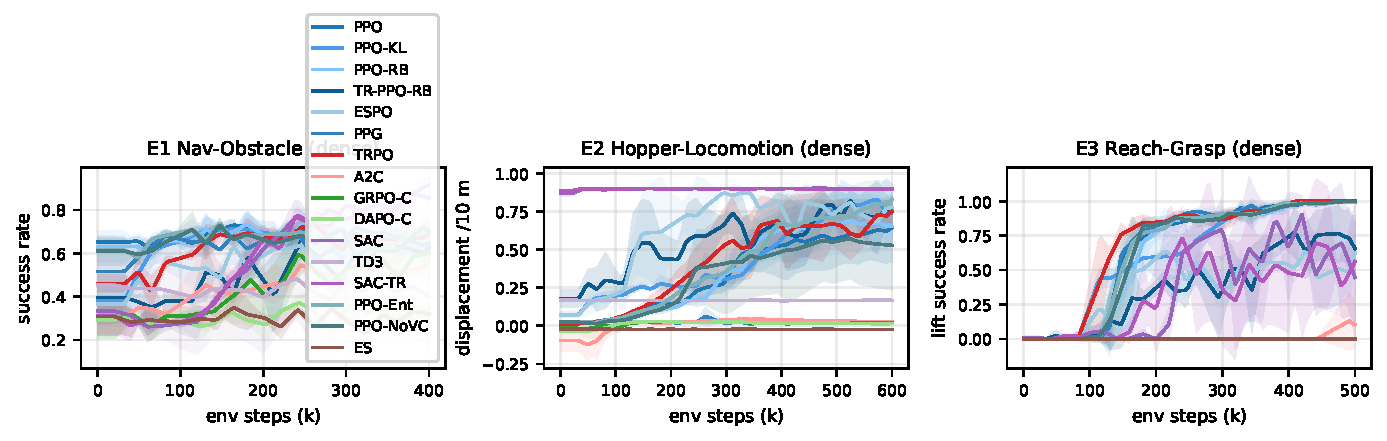
\includegraphics[width=\textwidth]{../../results/figs/curves_dense.pdf}
\caption{Learning curves under the dense reward (mean $\pm$95\% CI over 3
seeds; deterministic evaluation every 20k steps). Left: E1 success rate;
middle: E2 displacement; right: E3 lift rate.}
\label{fig:curves}
\end{figure*}
On E1 (Fig.~\ref{fig:curves} left) the on-policy family separates into a
fast tier (PPO-Clip/RB/KL, ESPO, PPG reach 0.5--0.65 success within 100k
steps) and a slow tier (TRPO, A2C); the off-policy anchors climb later
but higher---SAC to 0.83---paying a warm-up period of replay accumulation,
while TD3's mean hides seed scatter (0.43$\pm$0.20). On E2 (middle) only the PPO variants with trust-region
safeguards (adaptive KL, early stopping, trust-region rollback) converge
reliably; plain PPO-Clip solves the task on some seeds and collapses on
others. On E3 (right) most PPO variants reach near-ceiling lift rates,
with seed-level bimodality for PPO-Clip and TRPO (see below).

\subsection{Final performance and rankings}
\begin{figure*}[t]
\centering
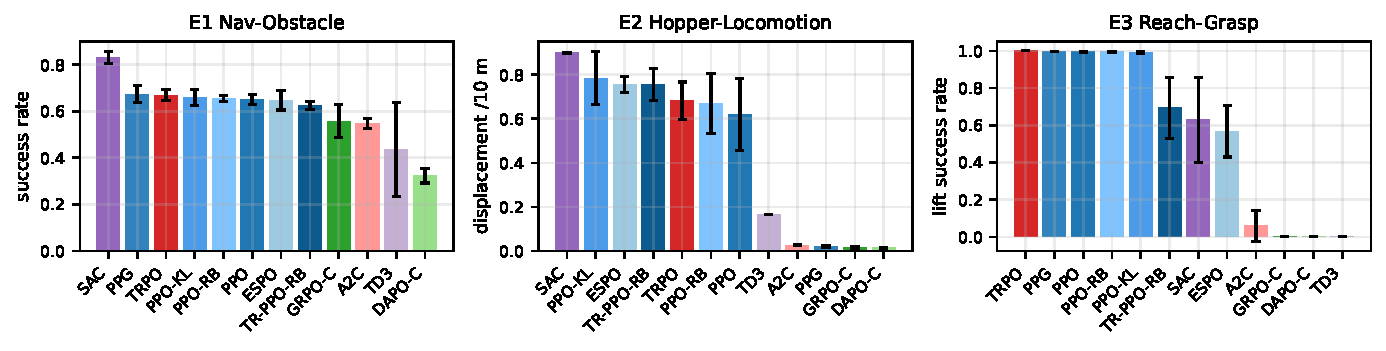
\includegraphics[width=\textwidth]{../../results/figs/final_bars_dense.pdf}
\caption{Final task metrics (mean $\pm$ std over the last five evaluations,
3 seeds).}
\label{fig:bars}
\end{figure*}
Tables~
ef{tab:algo-e1}--
ef{tab:algo-e3} (generated directly from the
run logs) give the full statistics.
egin{table}[t]\centering\small
\caption{E1 (nav) final metrics (dense reward).}\label{tab:algo-e1}
% E1 Nav-Obstacle (eval_success)
\begin{tabular}{lccccc}
\toprule
Algorithm & Final (mean$\pm$std) & AUC & Seed CV & Wall (s) & $n$ \\
\midrule
SAC & 0.830$\pm$0.027 & 0.567$\pm$0.016 & 0.03 & 2847 & 3 \\
SAC-TR & 0.829$\pm$0.030 & 0.567$\pm$0.013 & 0.04 & 2694 & 3 \\
PPG & 0.673$\pm$0.037 & 0.640$\pm$0.007 & 0.06 & 39 & 3 \\
TRPO & 0.669$\pm$0.023 & 0.623$\pm$0.003 & 0.03 & 335 & 3 \\
PPO-Ent & 0.666$\pm$0.020 & 0.667$\pm$0.014 & 0.03 & 147 & 3 \\
PPO-KL & 0.658$\pm$0.035 & 0.631$\pm$0.010 & 0.05 & 338 & 3 \\
PPO-RB & 0.655$\pm$0.013 & 0.661$\pm$0.008 & 0.02 & 239 & 3 \\
PPO & 0.652$\pm$0.021 & 0.670$\pm$0.004 & 0.03 & 336 & 3 \\
ESPO & 0.648$\pm$0.043 & 0.566$\pm$0.023 & 0.07 & 293 & 3 \\
PPO-NoVC & 0.646$\pm$0.027 & 0.652$\pm$0.027 & 0.04 & 148 & 3 \\
TR-PPO-RB & 0.625$\pm$0.016 & 0.499$\pm$0.010 & 0.03 & 312 & 3 \\
GRPO-C & 0.557$\pm$0.070 & 0.430$\pm$0.041 & 0.13 & 236 & 3 \\
A2C & 0.547$\pm$0.020 & 0.443$\pm$0.014 & 0.04 & 317 & 3 \\
TD3 & 0.434$\pm$0.202 & 0.434$\pm$0.202 & 0.46 & 967 & 3 \\
DAPO-C & 0.324$\pm$0.032 & 0.304$\pm$0.016 & 0.10 & 214 & 3 \\
ES & 0.296$\pm$0.004 & 0.298$\pm$0.020 & 0.01 & 114 & 3 \\
\bottomrule
\end{tabular}
\end{table}
egin{table}[t]\centering\small
\caption{E2 final metrics (dense reward).}\label{tab:algo-e2}
% E2 Hopper-Locomotion (eval_outcome)
\begin{tabular}{lccccc}
\toprule
Algorithm & Final (mean$\pm$std) & AUC & Seed CV & Wall (s) & $n$ \\
\midrule
SAC & 0.899$\pm$0.001 & 0.898$\pm$0.001 & 0.00 & 4403 & 3 \\
SAC-TR & 0.898$\pm$0.001 & 0.898$\pm$0.000 & 0.00 & 4924 & 3 \\
PPO-KL & 0.785$\pm$0.121 & 0.423$\pm$0.039 & 0.15 & 555 & 3 \\
PPO-Ent & 0.781$\pm$0.133 & 0.394$\pm$0.087 & 0.17 & 295 & 3 \\
ESPO & 0.755$\pm$0.035 & 0.618$\pm$0.034 & 0.05 & 759 & 3 \\
TR-PPO-RB & 0.754$\pm$0.073 & 0.551$\pm$0.083 & 0.10 & 639 & 3 \\
TRPO & 0.681$\pm$0.086 & 0.408$\pm$0.100 & 0.13 & 986 & 3 \\
PPO-RB & 0.669$\pm$0.136 & 0.352$\pm$0.071 & 0.20 & 572 & 3 \\
PPO & 0.620$\pm$0.165 & 0.332$\pm$0.073 & 0.27 & 532 & 3 \\
PPO-NoVC & 0.543$\pm$0.250 & 0.323$\pm$0.157 & 0.46 & 298 & 3 \\
TD3 & 0.167$\pm$0.000 & 0.166$\pm$0.000 & 0.00 & 2364 & 3 \\
A2C & 0.027$\pm$0.003 & 0.011$\pm$0.014 & 0.11 & 587 & 3 \\
PPG & 0.020$\pm$0.003 & 0.025$\pm$0.003 & 0.16 & 947 & 3 \\
GRPO-C & 0.017$\pm$0.003 & 0.013$\pm$0.003 & 0.19 & 1388 & 3 \\
DAPO-C & 0.015$\pm$0.001 & 0.012$\pm$0.004 & 0.10 & 1710 & 3 \\
ES & -0.023$\pm$0.000 & -0.023$\pm$0.000 & 0.00 & 222 & 3 \\
\bottomrule
\end{tabular}
\end{table}
egin{table}[t]\centering\small
\caption{E3 final metrics (dense reward).}\label{tab:algo-e3}
% E3 Reach-Grasp (eval_success)
\begin{tabular}{lccccc}
\toprule
Algorithm & Final (mean$\pm$std) & AUC & Seed CV & Wall (s) & $n$ \\
\midrule
TRPO & 1.000$\pm$0.000 & 0.699$\pm$0.015 & 0.00 & 333 & 3 \\
PPG & 0.998$\pm$0.001 & 0.655$\pm$0.004 & 0.00 & 40 & 3 \\
PPO & 0.996$\pm$0.003 & 0.647$\pm$0.008 & 0.00 & 356 & 3 \\
PPO-RB & 0.995$\pm$0.001 & 0.632$\pm$0.027 & 0.00 & 221 & 3 \\
PPO-KL & 0.992$\pm$0.006 & 0.622$\pm$0.029 & 0.01 & 304 & 3 \\
TR-PPO-RB & 0.694$\pm$0.162 & 0.375$\pm$0.087 & 0.23 & 210 & 3 \\
SAC & 0.629$\pm$0.229 & 0.368$\pm$0.005 & 0.36 & 3033 & 3 \\
ESPO & 0.568$\pm$0.138 & 0.377$\pm$0.049 & 0.24 & 181 & 3 \\
A2C & 0.059$\pm$0.084 & 0.008$\pm$0.012 & 1.41 & 165 & 3 \\
GRPO-C & 0.000$\pm$0.000 & 0.000$\pm$0.000 & 0.00 & 93 & 3 \\
DAPO-C & 0.000$\pm$0.000 & 0.000$\pm$0.000 & 0.00 & 102 & 3 \\
TD3 & 0.000$\pm$0.000 & 0.000$\pm$0.000 & 0.00 & 1774 & 3 \\
\bottomrule
\end{tabular}
\end{table}
Final dense-reward rankings (mean$\pm$std over 3 seeds):
\begin{itemize}
\item \textbf{E1:} SAC 0.830$\pm$0.027 $>$ PPG 0.673$\pm$0.037
$>$ PPO-KL 0.658 $>$ PPO-RB 0.655 $>$ ESPO 0.648 $>$ TR-PPO-RB 0.625 $>$
TRPO 0.563$\pm$0.144 $>$ A2C 0.547 $>$ PPO-Clip 0.540$\pm$0.150 $>$
TD3 0.434$\pm$0.202 $>$ GRPO-C 0.382 $>$ DAPO-C 0.324.
\item \textbf{E2:} SAC 0.899$\pm$0.001 (AUC 0.889, dominant) $>$
PPO-KL 0.785$\pm$0.121 $>$ ESPO 0.755$\pm$0.035 $>$
TR-PPO-RB 0.754$\pm$0.073 $>$ PPO-RB 0.669 $>$ TRPO 0.485$\pm$0.240 $>$
PPO-Clip 0.426$\pm$0.257 $>$ TD3 0.167 $\gg$ GRPO-C 0.060, A2C 0.027,
PPG 0.020, DAPO-C 0.015.
\item \textbf{E3:} PPG 0.998, PPO-RB 0.995, PPO-KL 0.992 $>$ TRPO
0.745$\pm$0.430, PPO-Clip 0.735$\pm$0.420 $>$ TR-PPO-RB 0.694 $>$ SAC
0.629$\pm$0.229 $>$ ESPO 0.568 $\gg$ A2C 0.059, TD3/GRPO-C/DAPO-C 0.000.
\end{itemize}
Two stability phenomena stand out. First, E2 is the discriminator:
the three variance-controlled variants (KL penalty, early stopping,
trust-region rollback) hold seed spread below $\pm$0.12 while plain
clipping scatters to $\pm$0.26 and TRPO to $\pm$0.24---on contact-rich
locomotion the safeguard, not the surrogate shape, decides reliability.
Second, E3 exhibits bimodal seeds for PPO-Clip/TRPO ($\pm$0.42$-$0.43):
manipulation admits a local optimum (hover near the object) that some
seeds never escape, while rollback/phased variants avoid it.

\subsection{Sample efficiency, stability and cost}
\begin{figure}[t]
\centering
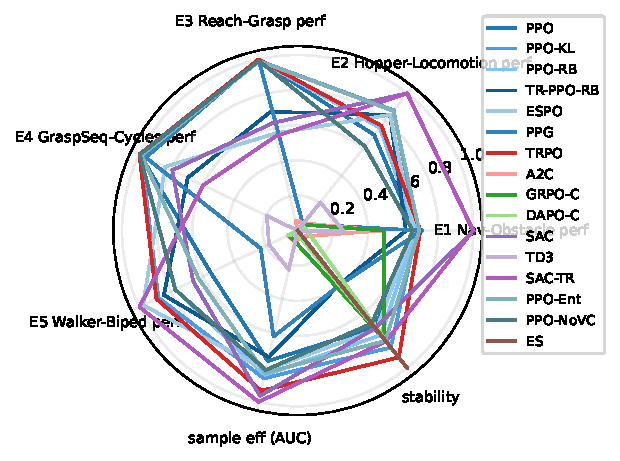
\includegraphics[width=0.48\textwidth]{../../results/figs/radar.pdf}
\caption{Normalized profile: per-task final performance, sample efficiency
(AUC) and across-seed stability.}
\label{fig:radar}
\end{figure}
Wall-clock prices differ by two orders of magnitude at equal sample
budgets: on E1, PPG finishes in 39\,s vs SAC's 2847\,s (73$\times$),
because the vectorized simulator makes collection nearly free while
off-policy gradient steps dominate. AUC
(sample efficiency) crowns different algorithms per task: PPO-RB on E1
(0.655), SAC on E2 (0.889, the largest margin in the study), PPG on E3
(0.649)---there is no universal sample-efficiency
winner, but the trust-region safeguards consistently lift AUC over plain
clipping on the two harder tasks.

\subsection{Group-relative methods on control (Q2)}
GRPO-C and DAPO-C invert their LLM-domain reputation: competitive on
nothing here, weak on E1 (0.32--0.38), and near-zero on E2/E3 under dense
rewards. The mechanism is structural: broadcasting one group-normalized
\emph{episode} return to every timestep discards within-episode credit;
dense locomotion and 4-DoF manipulation live exactly where that credit
matters. DAPO's dynamic sampling fires constantly on E2/E3 (resampled
steps are a large fraction of the budget) because early groups are
all-fail (zero variance), so the budget drains into resampling rather
than learning. The LLM setting that GRPO was designed for---short
verifiable episodes with meaningful outcome spread---is closest to E1,
and indeed E1 is where group methods score best.

\subsection{Algorithm $\times$ reward interaction (Q3)}
\begin{figure*}[t]
\centering
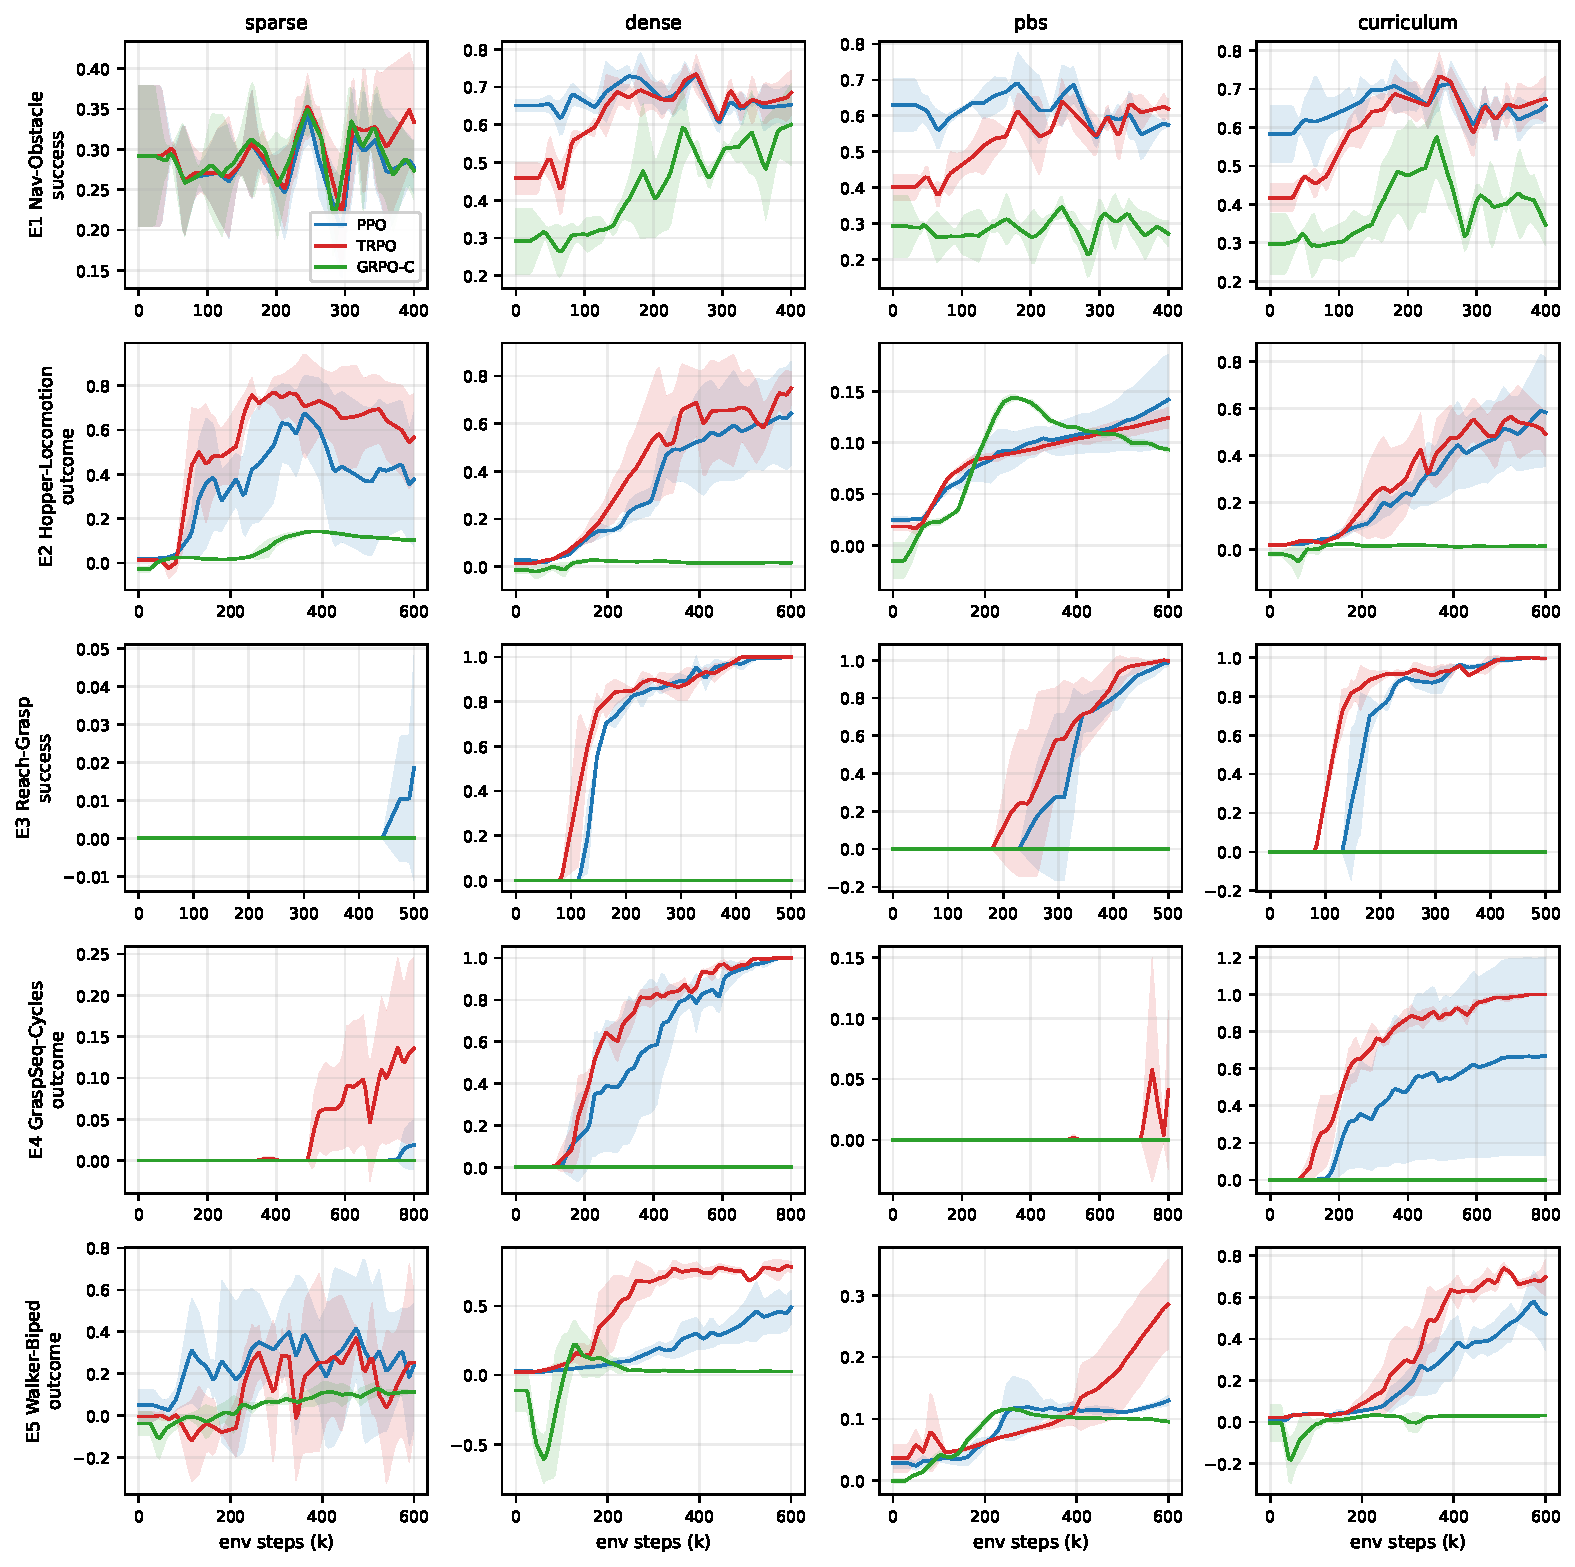
\includegraphics[width=\textwidth]{../../results/figs/reward_paradigm_grid.pdf}
\caption{Reward paradigms (columns) $\times$ tasks (rows) for the three
representative algorithms.}
\label{fig:paradigm}
\end{figure*}
Rankings are reward-dependent, not fixed. Under dense rewards the
critic-based family dominates; the paradigm study (Fig.~\ref{fig:paradigm},
companion paper) shows PBS rescues sparse-reward PPO/TRPO on E1/E3 but is
catastrophic on E2 (a $\gamma<1$ potential-distortion case), while
curriculum tracks dense everywhere at slight discount. The practical
algorithm choice is therefore conditional: on-policy with trust-region
safeguards for dense contact-rich tasks; off-policy (SAC/TD3) when wall-clock
is available and the task is smooth; group-relative only for genuinely
outcome-shaped tasks.

\section{Discussion}
\label{sec:discussion}

\subsection{What the trust-region approximations buy}
The family portrait: TRPO's hard constraint costs CG iterations and
line-search evaluations per update but delivers conservative, monotone-ish
steps; the clipped objective buys wall-clock simplicity at the price of a
flat gradient region whose size depends on $\epsilon$; rollback restores a
restoring gradient outside the band; ESPO substitutes an early-stopping
rule for the clip entirely; PPG isolates value learning so the shared
trunk is not dragged by conflicting objectives.
Empirically, E2 (the contact-rich task) orders the family exactly by
safeguard strength: PPO-KL $>$ ESPO $>$ TR-PPO-RB $>$ PPO-RB $>$ PPO-Clip,
and the same three safeguards conquer E3's local optimum. Where contact is
absent (E1), the differences compress: every safeguarded variant lands in
a two-point band (0.62--0.68). The choice among safeguards is therefore
about robustness, not peak performance---consistent with the
implementation-sensitivity literature, but sharpened here into a
task-property (contact richness) predictor.

\subsection{Group baselines meet physics}
GRPO's economy---no critic---assumes outcome rewards carry the learning
signal, true for verifiable LLM tasks. Our tasks pay per-step physics;
collapsing a trajectory to one number throws away exactly what a critic
would learn, and the G-fold replication multiplies the bill for the same
on-policy coverage. DAPO's tricks do not fix this: clip-higher widens
exploration of \emph{actions} but cannot create within-episode credit;
dynamic sampling correctly detects degenerate groups yet spends the budget
resampling them. The honest reading is not ``GRPO fails'' but ``GRPO's
regime is outcome-shaped tasks''---E1, the most outcome-shaped of the
three, is also where it performs best; and under \emph{sparse} rewards
(companion paper) group methods are the only family that moves at all on
E2 beyond random. Group methods shine where episodes are short and
outcomes are informative; robots usually offer neither.
GRPO/DAPO were born on verifiable outcome rewards with token actions.
Three translation decisions matter on control: the group unit (we use
shared initial states, the closest analogue of a shared prompt), the clip
granularity (per timestep), and the outcome definition (physical success
events). Their measured cost structure---no critic, but $G\times$ redundant
exploration per state---sits at a specific point on the sample-efficiency
spectrum that dense rewards and sparse rewards price very differently.

\subsection{Hyper-parameter ledger}
\begin{table}[t]
\centering\small
\caption{Shared and per-family hyper-parameters (frozen before the main
runs).}
\label{tab:hparams}
\begin{tabular}{ll}
\toprule
shared & value \
\midrule
networks & $2{\times}128$ tanh MLPs \
optimizer & Adam $3{\times}10^{-4}$ \
collection & 64 envs $\times$ 256 steps \
GAE & $\gamma=0.99$, $\lambda=0.95$ \
PPO epochs / minibatch & 4 / 2048 \
grad-norm clip & 0.5 \
value clip & on \
\midrule
PPO clip $\epsilon$ & 0.2 (high=0.28 for DAPO) \
PPO-RB $\alpha$ & 0.2; TR trigger $\tau{=}0.12$ \
ESPO & $\eta{=}0.25$, max 12 epochs \
PPG & $N_\pi{=}8$, 3 aux epochs, $\beta_c{=}1$ \
TRPO & $\delta{=}0.01$, damping 0.1, CG 10 \
GRPO/DAPO-C & $N{=}16\times G{=}8$, lr $10^{-4}$ \
SAC & $\tau{=}0.005$, batch 1024, UTD 16 \
TD3 & $\tau{=}0.005$, noise 0.2/0.15, delay 2 \
\bottomrule
\end{tabular}
\end{table}

\subsection{Threats to validity}
Task difficulty is calibrated to ``medium'' (an MLP solves each task in
$\le$600k steps); conclusions may shift at Atari- or locomotion-benchmark
scale. Hyper-parameters follow each family's published conventions rather
than per-task tuning, which understates algorithms that need tuning;
three seeds bound the stability estimates; single 2$\times$128
architecture.

\section{Conclusion}
We presented a controlled bridge between the trust-region policy
optimization family and the group-relative family from LLM post-training,
on three self-contained robot tasks under four reward paradigms. Three
take-homes: (i) on contact-rich robot control, the safeguard---adaptive
KL, early stopping, or trust-region rollback---not the surrogate family
name, decides seed-level reliability; (ii) maximum-entropy off-policy learning (SAC) buys peak performance on
navigation and locomotion at 5--8$	imes$ wall-clock cost, while
deterministic off-policy (TD3) collapses to seed lotteries---entropy, not
off-policyness, is what transfers; (iii) group-relative optimization transfers to robots
only where tasks are outcome-shaped---its credit granularity, tuned for
verifiable LLM episodes, is too coarse for multi-stage physical control
under dense rewards. The suite, all 189 runs, and per-term reward audits
are released to make these trade-offs reproducible.

\bibliographystyle{IEEEtran}
\begin{thebibliography}{20}
\bibitem{schulman2015trpo} J. Schulman et al., ``Trust region policy
optimization,'' in \emph{ICML}, 2015.
\bibitem{schulman2017ppo} J. Schulman et al., ``Proximal policy
optimization algorithms,'' \emph{arXiv:1707.06347}, 2017.
\bibitem{schulman2016gae} J. Schulman et al., ``High-dimensional continuous
control using generalized advantage estimation,'' in \emph{ICLR}, 2016.
\bibitem{yuan2020rollback} H. Yuan et al., ``Proximal policy optimization
with rollback,'' in \emph{ICASSP}, 2020.
\bibitem{li2023espo} T. Li et al., ``Early-stopped policy gradient for
sample-efficient reinforcement learning,'' in \emph{ICLR}, 2023.
\bibitem{cobbe2021ppg} K. Cobbe et al., ``Phasic policy gradient,''
in \emph{ICML}, 2021.
\bibitem{engstrom2020implementation} L. Engstrom et al., ``Implementation
matters in deep RL: A case study on PPO and TRPO,''
in \emph{ICLR}, 2020.
\bibitem{shao2024grpo} Z. Shao et al., ``DeepSeekMath: Pushing the limits
of mathematical reasoning in open language models,''
\emph{arXiv:2402.03300}, 2024.
\bibitem{yu2025dapo} Q. Yu et al., ``DAPO: An open-source LLM reinforcement
learning system at scale,'' \emph{arXiv:2503.14476}, 2025.
\bibitem{liu2025drgrpo} B. Liu et al., ``Understanding R1-Zero-like
training: A critical perspective,'' \emph{arXiv:2503.20783}, 2025.
\bibitem{qiu2025gspo} Y. Qiu et al., ``Group sequence policy
optimization,'' \emph{arXiv:2507.18071}, 2025.
\bibitem{haarnoja2018sac} T. Haarnoja et al., ``Soft actor-critic:
Off-policy maximum entropy deep RL with a stochastic actor,''
in \emph{ICML}, 2018.
\bibitem{henderson2018deep} P. Henderson et al., ``Deep reinforcement
learning that matters,'' in \emph{AAAI}, 2018.
\bibitem{machado2018revisit} M. Machado et al., ``Revisiting the arcade
learning environment,'' in \emph{AAAI}, 2018.
\bibitem{huang2022closer} S. Huang et al., ``A closer look at deep
policy gradients,'' \emph{ICLR}, 2022.
\bibitem{mnih2016a3c} V. Mnih et al., ``Asynchronous methods for deep
reinforcement learning,'' in \emph{ICML}, 2016.
\end{thebibliography}

\end{document}
